\chapter{Zusammenfassung, \\ Disskusion \\ und Kritik}
\label{Disskusion}

Im letzen Teil dieser Auswertung wollen wir nochmal alles auf den Puntkgebracht Zusammenfassen, die Ergebnisse diskutieren und Kritik, 
bzw. Fehlerquellen analisieren und Verbesserungen überlegen.
Dafür Teilen wir die Auswertung verschiedene Teile ein, einmal einen, der die bestimmten Ricdhtmomnete $D_G$ und $D_R$ vergleicht, wie gut die Bestimmung des Schwerpunktes lief
und Zuletzt, wie nah wir an den Satz von Stein gekommen sind.

\section{Graphische oder rechnerische Auswertung?}
Wir mussten in den Aufgaben 1 und 2 das Richtmoment der Torsionsfeder bestimmen. In Aufgabe 1 wurde dies graphisch Gemacht, über eine statische Auslenkung, in der zweiten dann rechnerisch über die Schwingdauer.
Dabei kamen wir auf Ergebnisse für \hyperref[e:d_g]{$D_G$ (3.18)} und \hyperref[e:d_r]{$D_R$ (3.32)}:
\begin{align}
    D_G &= (4,3 \pm 0,5) \, &&10^{-2} \frac{Nm}{rad}\\
        \notag \\
    D_R &= (2,29 \pm 0,06) \, &&10^{-2} \frac{Nm}{rad}.
\end{align}

Mit beiden wurde in den Folge Aufgaben gerechnet, um die Ergebnisse auch dort zu vergleichen. Denn welcher Wert tatsächlich den >>Literaturwert<<
der Feder annimmt, ist anhand der Methoden nicht zu bestsimmen. Jedoch können wir schauen, ob sich nicht beiden Werte in einer 1-$\sigma$-Umgebung befinden und somit beide >>gleich richtig<< sind.
Daher nutzen wir \hyperref[eq:signifikante_abweichung]{die Berechnung der signifikanten Abweichung}:
\begin{equation}
    \sigma = \frac{\left| 0,043 - 0,0229 \right|}{\sqrt{(0,005)^2+(0,0006)^2}} = 3,99\sigma.
\end{equation}

Diese Abweiung ist gigantisch und scheint fast zwei verschiedene Federn zu beschreiben. Von statistischer Signifikanz darf man hier wirklich nicht sprechen. Aber wie kann das sein?
Vermutlich ist die plausibelste Begründung, dass der Fehler bei der graphischen Berechnung liegt. Sowohl wird die Ausgleichsgerade nicht optimal liegen, zudem ist die Skala in ihrer Präzision sehr limitiert,
wodurch sich hier viele enorme Ungenauigkeiten eingebunden haben könnten. Also ist die Ungenauigkeit nicht nur auf die Messgenauigkeit bezogen, sondern sogar auf die Auswertugnsmethode selbst. 
Das unterscheidet die graphische von der rechnerischen Methode, welche alleinig der Messungenauigkeiten unterliegt. Jedoch wurden zwei verschiedene Messmethoden verwendet, wodurch es nicht klar 
ausgeschlossen werden kann, dass nicht dennoch der graphische Wert der akkuratere ist. Es lässt isch nur sagen, dass der rechnerische Wert in sich selbst genauer ist, da seine Ungenauigkeit um ca. einen Faktor $10$ kleiner ist.

Wie erwähnt, wurden beide Werte zur Bestimmung der Trägheitsmomente in den letzten Aufgaben verwendet. Der Fehler hat sich logischer weise durchgezogen. Wir vergleichen nochmal \hyperref[e:s_t]{die Ergebnisse (43 und 44)} der Trägheitsmomente:
\begin{align}
    J_{P,G} &= (39,022 \pm 0,018)\, &&\mathrm{10^{-4}kg \, m^2} \\
        \notag \\
    J_{P,R} &= (26,3170 \pm 0,0017 )\, &&\mathrm{10^{-4} kg \, m^2}.
\end{align}

Wir schauen uns hier wieder \hyperref[eq:signifikante_abweichung]{die Berechnung der signifikanten Abweichung} an:
\begin{equation}
    \sigma = \frac{\left| 0,0039022 - 0,0026317\right|}{\sqrt{(0,0000018)^2 + (0,00000017)^2}} = 702,71\sigma.
\end{equation}

Diese Abweichung ist unglaublich groß. Dies liegt insbesondere daran, dass wir enorm kleine Ungenauigkeiten haben. Es zeigt sich damit insbesondere aber, dass es wichtig gewesen wäre, das Richtmoment $D$ exakter 
zuvor bestimmt zuhaben, damit sich die Ungenauigkeit in weiteren Berechnungen nicht durch zieht.

Zumschluss wollen wir zum Vergleich der bediden Methoden nochmal den Steinischen Satz schauen und hier wird sich etwas bemerkenswertes herausstellen. Zunächst nutzen wird \hyperref[eq:arithmetisches_mittel]{das arithmetische Mittel}, um die durchschnittlichen Abweichungen 
der berechnetetn Trägheitsmomente mit und ohne den Stein'schen Satz und tuen dies für die graphische und die rechnerische Methode:
\begin{align}
    \bar{\sigma}_G = 0,338\sigma \\
    \bar{\sigma}_R = 0,1842\sigma.
\end{align}

In beiden fällen ist der Stein'sche Staz im Mittel statistisch signifikant, jedoch ist der Wert der Rechnerischen Methode definitv näher am Satz von Stein. 
Bei beiden Methoden ist der Trend zu beobnachten, dass die Werte für größere Abstände eine größere $\sigma$-Abweichung aufweisne, was Vermutlich auf das quadrieren des Radiuses zurückzuführen ist, da der Fehler dadurch immer größer wird.
Jedoch befinden sich alle Werte der rehcnerischen Methode im 1-$\sigma$-Berecih, während der letzte Wert der graphsciehn Methode um über 1,1-$\sigma$ abweicht und somit nicht mehr als pauschal statistisch signifikant angenommen werden sollte.

Als Fait lässt sich sagen, dass die rechnerische Ermittlung des Richtmomentes die vermutlich akkuratere ist, denn der Fehler ist kleiner, und physikalische Gesetzte lassen sich akkurater damit reproduzieren.
Jedoch ist dies keine Garantie, dass der rechnerische Wert der tatsächlich akkuratere ist.

\section{Bestimmung des Schwerpunktes}
Diese Aufgabe war keine besonders große. Es ist eine sehr ungenaue Bestimmung des Schwerpunktes, denn dieser wrude über eine sehr grobe Methode bestimmt. Man hätte das Vorgehen auch anders machen können:
hätte man den Messingkörßer zweimal in verschiedenen Ausrichtungen über einen Faden an die Wand gehängt und an dem selben Punkt, wo der Faden an der Wand befestigt ist einen dünnen Faden genommen und den über den Messingkörper gehängt,
so hätte man wieder zwei Geraden ziehen können (entlang des dünnen Fadens) und deren Schnittpunkt als Schwerpunkt approximieren können. Diese Methode wäre vermutlich genauer, da sie nicht auf menschliche Feinmotorik setzt, sondern 
auf die Gravitation der Erde, welche frei von menschlichem Versagen ist. Wir haben hier jedoch keinen Wert zum kritiesieren und auswerten, da wir den Schwerpunkt rein qualitativ approximiert haben.

\section{Gültgkeit des Stein'schen Stazes}
Im letzen Teil wollen wir nochmal die Aussage Kraft des Stein'schen Satzes begut achte, auch wenn das meiste im Teil >>Graphische oder rechnerische Auswertung?<< bereits besprochen wurde. 
Wir werden uns daher auch nur auf die Werte berufen, die über das rechnerisch-bestimmte Richtmoment berechnet wurden. 
Denn wie bereits erwähnt, wurden die Werte der rechnerischen Methode immer ungenauer, wobei nur die Achse $a_4$ eine Ausnahme stellt, dieser Wert wurde wieder genauer. Dies liegt vermutlich an den Messmethoden, die durch menschliche Ungenauigkeiten hervorgerufen wurden.
Insbesondere hat der quadratische Abstand einen enormen Einfluss und wird die Werte nach hinten hinaus immer ungenauer machen. 
In einem simplen Pthon-code habe ich die Wetre in einem Balkendiagramm dargestellt und deren prozentuale Entwicklung berechnet:
\begin{figure}[h!]
    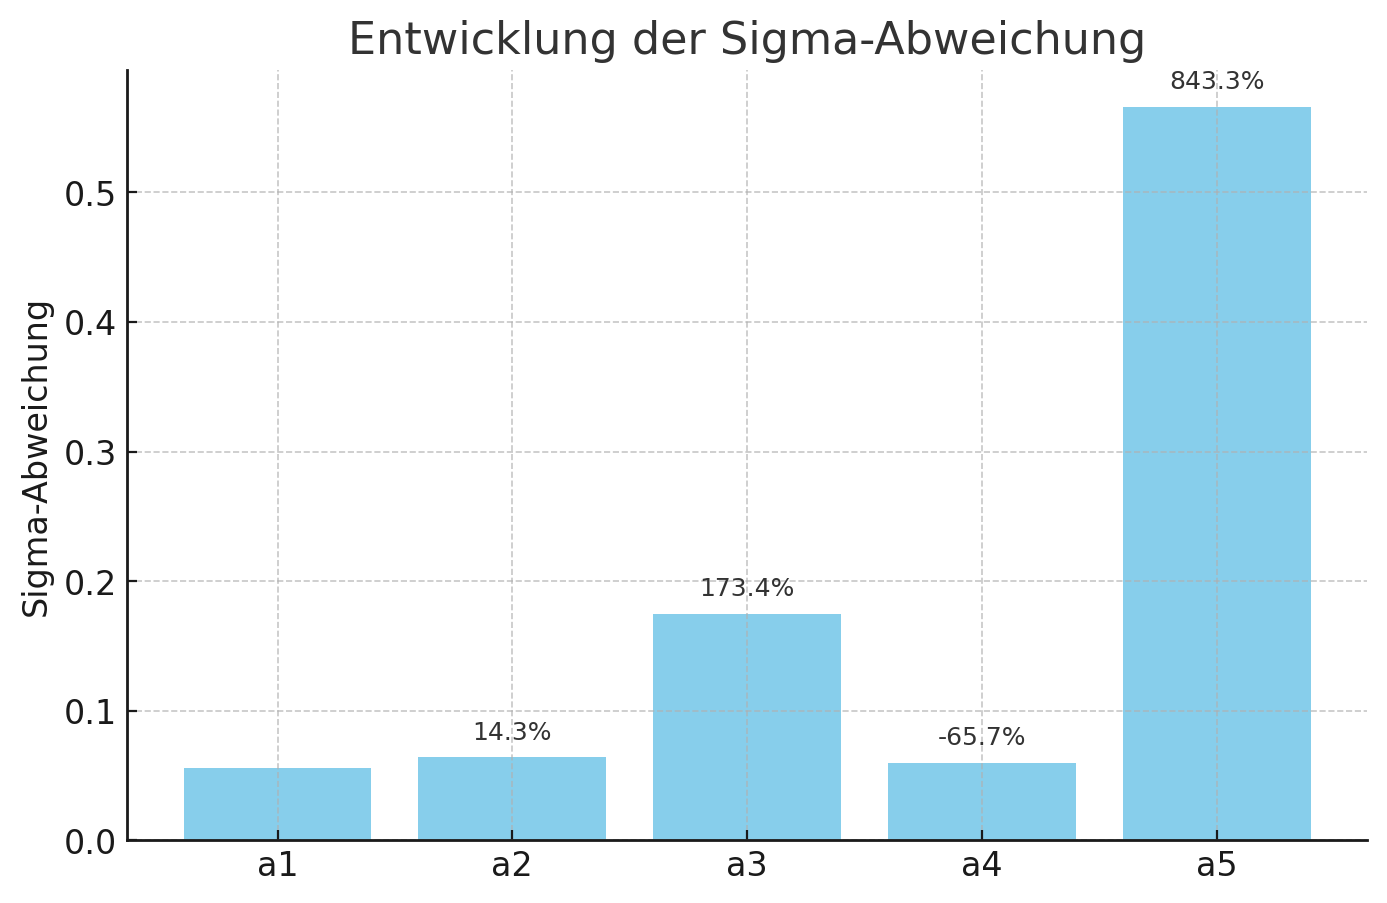
\includegraphics[width=0.45\textwidth]{img/\versuchsnummer/Balken_sigma.png}
    \caption{Prozentuale Entwicklung der $\sigma$-Abweichungen.}
    \label{img:balken_sigma}
\end{figure}

Unschwer zu erkennen ist ein Wachstum, dass vermutlich quadratisch ist. Jedoch sind es zu wenig Werte, um die Aussage dessen Experimentell klar behaupten zukönnen. Aus den mathematischen Gleichungen heraus jedoch, lässt sich dies ablesen.
Der Wert $a_4$ stellt eine Aussnahme da, welcher nur über genauere und mehr Messwerte bereinigt werden könnte. 
Besonders wichtig ist aber vor allem, dass alle Werte sich in der 1$\sigma$ Umgebung befinden und damit als statistisch signifikant gelten und den steinischen Satz genau genug nähren.
